\documentclass[a4paper,12pt]{article}
\usepackage{times}
\usepackage[francais]{babel}
\usepackage[utf8]{inputenc}
\usepackage[T1]{fontenc}
\usepackage{amsmath}
\usepackage{amssymb}
\usepackage{graphicx}
\usepackage{pdfpages}
\usepackage{pdflscape}
\usepackage{listings}
\usepackage{longtable}
\usepackage{hyperref}
\lstset{literate=
{é}{{\'e}}1
{è}{{\`e}}1
{ê}{{\^e}}1
{à}{{\`a}}1
{â}{{\^a}}1
}
\lstset{language=C++,
                basicstyle=\footnotesize,
                keywordstyle=\footnotesize\color{blue},
                otherkeywords={override,nullptr}
}
\definecolor{orange}{rgb}{0.8,0.4,0.0}
\definecolor{darkblue}{rgb}{0.0,0.0,0.6}
\definecolor{cyan}{rgb}{0.0,0.6,0.6}
\lstdefinelanguage{JSON}
{
  basicstyle=\normalsize,
  columns=fullflexible,
  showstringspaces=false,
  commentstyle=\color{gray}\upshape,
  morestring=[b]",
  morestring=[s]{>}{<},
  morecomment=[s]{<?}{?>},
  stringstyle=\color{orange},
  identifierstyle=\color{darkblue},
  keywordstyle=\color{blue},
  morekeywords={string,number,array,object}% list your attributes here
}

\sloppy

\setlength{\topmargin}{0cm}
\setlength{\headsep}{0.in}
\setlength{\headheight}{0.in}
\setlength{\evensidemargin}{0cm}
\setlength{\oddsidemargin}{-1cm}
\textwidth 18cm
\textheight 25cm

\begin{document}

\thispagestyle{empty}

\begin{titlepage}

\vspace*{2cm}

\begin{center}\textbf{\Huge Projet Logiciel Transversal}\end{center}{\Large \par}

\begin{center}\textbf{\large JAMET Romain DORRA Benjamin}\end{center}{\large \par}

\vspace{2cm}

%\begin{figure}[h]
%\begin{center}
%\includegraphics[width=\textwidth]{exemple.png}
%\caption{\label{pacmangame}Exemple du jeu}
%\end{center}
%\end{figure}

\clearpage

{\small
\tableofcontents
}

\end{titlepage}

\clearpage
\section{Présentation Générale}

\subsection{Archétype}
Le jeu d’origine est le jeu de stratégie/gestion Crusader Kings II, développé et édité par le studio Paradox Interactive. 

Il s’agit d’un jeu se déroulant dans l’Europe et le Moyen-Orient entre le VIIIe et le XVe siècle, où les joueurs jouent le rôle d’une dynastie de nobles régnant sur un domaine, qu’ils peuvent faire croitre par une mécanique de titres de noblesse, de guerre et de diplomatie inspirés du Moyen-Âge. 
Les règles en seront bien évidemment simplifiées dans le cadre du projet. 

Le descriptif des règles ci-dessous présente le projet tel qu’il devrait être au final. \\

\subsection{Règles du jeu}
Les joueurs sont des nobles qui règnent sur ces provinces, en possédant un ou plusieurs titres de noblesse. Les trois titres sont, dans l'ordre du plus puissant au moins puissant : les Rois, les Ducs, et les Comtes.

À chaque province est lié un titre de Comte. Posséder un titre de Comte, c'est posséder la province associée. 

Une province possède plusieurs caractéristiques décrivant son niveau de développement, son état de dévastation ou de prospérité, qui influent sur les impôts qu'elle génère, et les levées militaires qu'elle peut supporter. Un Comte peut posséder plusieurs Comtés, cependant, le nombre en est limité. Si cette limite est dépassée, un malus d’impôts et de levées est appliqué.  \\

Un Duc est plus puissant qu’un Comte. Pour pouvoir contrôler plus de territoire malgré la limite mentionnée précédemment, il doit confier la gestion de certaines provinces à des nobles qui seront ses vassaux. 

Un Duc ne peut avoir que des Comtes pour vassaux.

Un Roi est plus puissant qu’un Duc. Il peut avoir comme vassaux des Ducs et des Comtes.
Lorsqu’un seigneur est vassal, il paie un impôt en or et en hommes à son suzerain. \\

Pour faire la guerre à son voisin, il faut un Casus Belli. Il y aura la possibilité de dépenser de l’or pour fabriquer une revendication à un titre de Comte, pour essayer de s’en emparer à la guerre. Une fois la guerre déclarée, on peut mobiliser les troupes dans les provinces que l’on possède, ainsi que les troupes de ses vassaux si on en a, et leur donner des ordres de déplacement sur la carte.

Lorsque deux armées hostiles se rencontrent, un combat a lieu. L’armée défaite est mise en déroute et cherchera automatiquement à revenir à sa province d’origine. \\

Chaque Comté fait partie d’un Duché «de Jure », c’est-à-dire un Duché dont le titre n’existe pas, mais qui peut être créé si quelqu’un en contrôle plus de la moitié et dépense une certaine somme. Le fait de posséder un titre de Duc offre un Casus Belli permettant de vassaliser les Comtes dont les terres font partie « de Jure » de votre Duché.

De même, chaque Duché fait partie d’un Royaume de Jure. Posséder ou contrôler par le biais de vassaux une certaine proportion d’un Royaume de Jure vous permet de créer ce titre en échange d’argent. Posséder un tel titre offre un Casus Belli contre tous les Ducs et Comtes faisant partie de Jure de votre Royaume.
On peut bien évidemment posséder ou contrôler par vassaux des provinces n’appartenant pas de Jure à votre domaine. \\

Il est possible d’interagir avec d’autres personnages, forger des alliances, des pactes de non-agression, proposer à un seigneur plus faible de devenir votre vassal. 

Chaque personnage possède un score décrivant son opinion envers les autres, influencé par l’historique de leurs actions. Ce score permettra de définir le comportement de l’IA. Il sera également influencé par des traits de personnalité des personnages.
L’IA prendra ses décisions en utilisant une mécanique de MMTH (mean time to happen, ou temps moyen d’attente). Pour chaque action, il y a un MTTH en nombre de tours, avec des modificateurs liés aux traits de personnalité aléatoires des personnages.

Au cours de son règne, un personnage accumule des points de prestige selon la quantité de titres qu’il possède, ainsi que les titres de ses vassaux. Lorsqu’il meurt, un héritier apparaît, et le score de prestige s’ajoute au score du joueur. Le score final d’un joueur correspond donc à la somme de points de prestige accumulés par tous les seigneurs successifs qu’il a joué. \\


\subsection{Ressources}
Pour réaliser ce projet, nous aurons besoin en termes de ressources d’une carte du monde du jeu, avec les différentes provinces découpées. 

Nous aurons besoin d’une version pour l’affichage, et d’une autre qui ne sera pas affichée pour identifier la province sur laquelle le joueur clique, par un code couleur unique par province. \\

Nous aurons besoin de sprites d’armée immobile, en mouvement, et à la bataille. 

Nous devrons pouvoir coloriser facilement les bannières pour identifier immédiatement le contrôleur de l’armée. 

Nous pouvons également avoir besoin d’images pour les personnages, même si ce n’est pas obligatoire il s’agirait d’un plus. Dans le même ordre d’idées, nous pourrions employer diverses images sur le thème médiéval pour illustrer les différents menus du jeu. Nous pouvons aussi utiliser différentes musiques d’ambiance, des bruitages de bataille, et quelques sons génériques pour l’appui sur les boutons de l’interface. \\

\begin{figure}[hbtp]
\centering
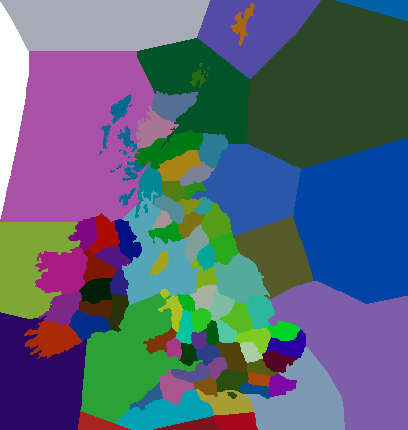
\includegraphics[width=0.4\textwidth]{ru.jpg}
\caption{royaume-uni} 
\end{figure}

\clearpage
\section{Description et conception des états}

L'état de jeu est contenu dans une classe principale : GameState, qui contient tous les éléments du jeu propres à l'état d'une partie de jeu.
Certains éléments de l'état de jeu ont besoin de références à d'autres éléments. Afin d'être compatible avec une exécution rapide en jeu et un système de sauvegarde sûr, les éléments auxquels il peut être fait référence sont dotés d'un champ id unique, qui sert à les identifier. Ainsi, pour référencer le personnage propriétaire d'un titre dans la classe Title on doit mettre l'id unique correspondant à ce personnage. Pour ce faire, on emploie des std::map qui associent id et objet.

\subsection{Description des états}

\begin{itemize}
\item GameState\\
Elle contient :
\begin{itemize}
\item un objet ressources de la classe Ressources, chargé de contenir toutes les ressources statiques servant au fonctionnement du jeu. 
\item un objet gameMap de la classe GameMap, décrivant l'état des éléments dynamiques de la carte, 
\item un objet politics de la classe Politics, décrivant l'organisation géopolitique de la partie. 
\item une liste de joueurs (players) de la classe std::vector<Player> pour suivre l'évolution des différents joueurs, humains ou IA.\\
\end{itemize}

\item Politics\\
La classe Politics décrit l'ensemble des entités politiques existantes. 
\begin{itemize}
\item On a d'abord la liste des titres (titles), de la classe Titles. Il s'agit de tous les titres qui existent ou peuvent être créés. 
\item On a ensuite la liste de tous les personnages (characters), de la classe Characters, qui contient tous les personnages en vie ou morts. 
\item Enfin, on a la liste de toutes les relations (relations) qui peuvent exister entre deux personnages (alliances, etc.), de la classe std::vector<Relation>. \\
\end{itemize}

\item Titles\\
La classe Titles décrit tous les titres qui existent ou peuvent être créés.
\begin{itemize}
\item un champ titleType de type enum, qui peut prendre la valeur kingdom, county, ou duchy,
\item un champ titles de type std::map<std::string, titleType>,
\item un champ kingdoms de type std::map<std::string, Kingdom>
\item un champ duchies de type std::map<std::string, Duchy>
\item un champ counties de type std::map<std::string, County>
\end{itemize}
\item Title\\
La classe Title décrit un titre de noblesse, que celui-ci soit possédé par quelqu'un ou non. Il contient
\begin{itemize}
\item un champ id de type std::string,
\item un champ nom(name) de type std::string,
\item un champ propriétaire (holder) de type std::string
\end{itemize}
De la classe Title, héritent les classes County, Duchy, Kingdom (Comté, Duché, Royaume). 

\item County\\
\begin{itemize}
\item un champ province de type std::string qui désigne la province associée au titre
\item un champ liege de type std::string qui désigne le suzerain
\item un champ deJureLiege de type std::string qui désigne le suzerain de jure
\end{itemize}
\item Duchy\\
\begin{itemize}
\item un champ liege de type std::string qui désigne le suzerain
\item un champ deJureLiege de type std::string qui désigne le suzerain de jure
\end{itemize}
\item Kingdom\\

\item Characters\\
\begin{itemize}
\item le champ characters de type std::map<std::string, Character>
\item un champ opinions de type std::vector<std::string, std::map<std::string, int>> qui contient les opinions d'un personnage sur les autres,
\end{itemize}
\item Character\\
La classe Character décrit les personnages du jeu. Les personnages peuvent posséder des titres, ont des statistiques, une opinion, des traits de caractère et peuvent mener des guerres ou comploter. Elle possède de nombreux attributs :
\begin{itemize}
\item un champ id de type std::string
\item un champ name de type std::string
\item un champ dynastyName de type std::string qui décrit la dynastie
\item un champ age de type int
\item un champ traits de type std::vector<std::string> qui contient les id des traits de caractère que possède le personnage
\item un champ diplomaty de type int qui décrit son talent diplomatique
\item un champ stewardship de type int qui décrit sa capacité à gérer les fiscalités de provinces
\item un champ martial de type int qui décrit son talent martial
\item un champ intrigue de type int qui décrit son talent pour les complots
\item un champ claims de type std::vector<std::string> qui décrit les revendications du personnage. Cela lui permet de déclarer la guerre pour récupérer un titre sur lequel il a des revendications.
\item un champ alive de type bool
\item un champ prestige de type int qui décrit le score du personnage
\item un champ gold de type int
\item un champ plotTypes, énumération qui regroupe {none, claim, murder}
\item un champ hasPlot de type bool qui décrit si le personnage a ou non un complot en cours
\item un champ plotTarget de type std::string qui donne l'id de la cible d'un hypothétique complot, cette cible pouvant être un personnage ou un titre selon le type de complot.
\item un champ plotType de type plotTypes qui décrit le type de complot (au plus un) mené actuellement par le personnage.
\item un champ plotEnd de type int qui décrit le tour où le complot en cours se termine.\\
\end{itemize}

\item Relation\\
La classe Relation décrit un lien particulier entre deux personnages actifs (vivants). Elle contient 
\begin{itemize}
\item un champ characterA et 
\item un champ characterB, tous deux de type std::string,
\item une énumération relType qui peut valoir : {non\_aggression, alliance, friendship, rivalry, war} et désigne les types de relation possibles,
\item un champ type de type relType qui désigne le type de relation qui existe entre deux personnages,
\item une date (numéro de tour) de fin (endTurn) qui vaut 0 dans le cas d'une durée indéterminée.\\
\end{itemize}

\item Player\\
La classe Player décrit un joueur (humain ou IA).
Les champs sont :
\begin{itemize}
\item id de type std::string
\item currentCharacter de type std::string qui décrit le personnage actuellement contrôlé
\item score de type int qui décrit  le score total du joueur
\end{itemize}
\item AIPlayer\\
Une sous-classe de Player.
\item HumanPlayer\\
Une sous-classe de Player.\\

\item Ressources\\
La classe Ressources décrit les ressources statiques utilisées par le jeu. Elle contient les champs suivants :
\begin{itemize}
\item un champ traits de type Traits qui contient tous les traits de caractère que peuvent avoir les personnages
\item un champ adjacencies de type Adjacencies qui contient le nombre de tours nécessaires à une armée pour passer d'une province à une autre.\\
\end{itemize}

\item Adjacencies\\
La classe Adjacencies regroupe le nombre de tours nécessaires pour passer d'une province à une autre dans le champ val de type std::map<std::string, std::map<std::string, int>>. Si les provinces ne sont pas adjacentes, la distance est 0. Entre une province et elle-même, la distance est -1.\\

\item Traits\\
Cette classe regroupe tous les traits de caractère que peut avoir un personnage dans le champ traits de type std::vector<Trait>.
\item Trait\\
Cette classe décrit un trait de caractère. Elle comprend :
\begin{itemize}
\item un champ id de type std::string
\item un champ opposedId de type std::string qui donne l'id du trait de caractère opposé
\item diplomacyModifier de type int qui décrit l'effet qu'a le trait sur la statistique diplomacy
\item stewardshipModifier de type int qui décrit l'effet qu'a le trait sur la statistique stewardship
\item martialModifier de type int qui décrit l'effet qu'a le trait sur la statistique martial
\item intrigueModifier de type int qui décrit l'effet qu'a le trait sur la statistique intrigue\\
\end{itemize}

\item GameMap\\
La classe GameMap décrit la situation des différentes zones, les batailles et les armées. 
Elle présente les champs suivants :
\begin{itemize}
\item un champ provinces de type std::map<std::string, Province> qui regroupe les différentes provinces.
\item un champ armies de type std::map<std::string, Army> qui regroupe les différentes armées.
\item un champ battles de type std::map<std::string, Battle> qui regroupe les différentes batailles.\\
\end{itemize} 

\item Battle\\
Les champs sont :
\begin{itemize}
\item id de type std::string
\item province de type std::string la province où a lieu la bataille
\item whiteArmies de type std::vector<std::string>
\item blackArmies de type std::vector<std::string>
\item startTurn de type int le tour de début de la bataille
\item endTurn de type int le tour de fin de la bataille\\
\end{itemize}

\item Army\\
Décrit une armée. Contient les champs : 
\begin{itemize}
\item id de type std::string
\item levies de type std::vector<std::string> les id des levées qui composent l'armée
\item currentProvince de type std::string la position actuelle de l'armée
\item currentBattle de type std::string la bataille actuellement menée par l'armée
\item orders de type std::queue<TravelOrder> les ordres que suit l'armée.
\end{itemize}
\item Order\\
Ordre donné à une armée. contient les champs :
\begin{itemize}
 \item originProvinceId de type std::string id de la province de départ
 \item destinationProvinceId de type std::string idée de la province d'arrivée
 \item duration de type int qui contient le temps total (en nombre de tours) nécessaire pour exécuter l'ordre
 \item elapsed de type int, le nombre de tours écoulés depuis que l'ordre a été donné.
 \end{itemize}
\item TravelOrder\\
Ordre des provinces par lesquelles passe une armée. Hérite de Order. Contient un champ de type std::vector <OneProvinceOrder> 
\item OneProvinceOrder\\
Hérite de Order. Détermine l'ordre de déplacement d'une armée province par province.\\

\item Province\\
Cette classe décrit une province. Elle comprend les champs suivants :
\begin{itemize}
\item id de type std::string
\item name de type std::string
\item colorCode de type unsigned int, identifiant de couleur unique qui permet d'identifier la province à sa position sur la carte.
\item development de type unsigned char
\item prosperity de type char qui détermine le niveau de prospérité de la province
\item baseLevy de type Levy la levée de base
\item levy de type Levy qui calcule la levée réelle après prise en compte de l'état de la province
\item baseTaxIncome de type unsigned int l'argent que la province rapporte de base
\item taxIncome de type unsigned int les impôts réels après prise en compte de l'état de la province
\end{itemize}
\item Levy\\
Décrit une levée.
\begin{itemize}
\item unsigned men de type int le nombre d'hommes dans la levée
\item isRaised de type bool qui décrit si la levée a été mobilisée
\item reinforcementRate de type float la vitesse de renouvellement de la levée
\end{itemize}
\end{itemize}

\subsection{Conception Logiciel}

\begin{landscape}
\begin{figure}[p]
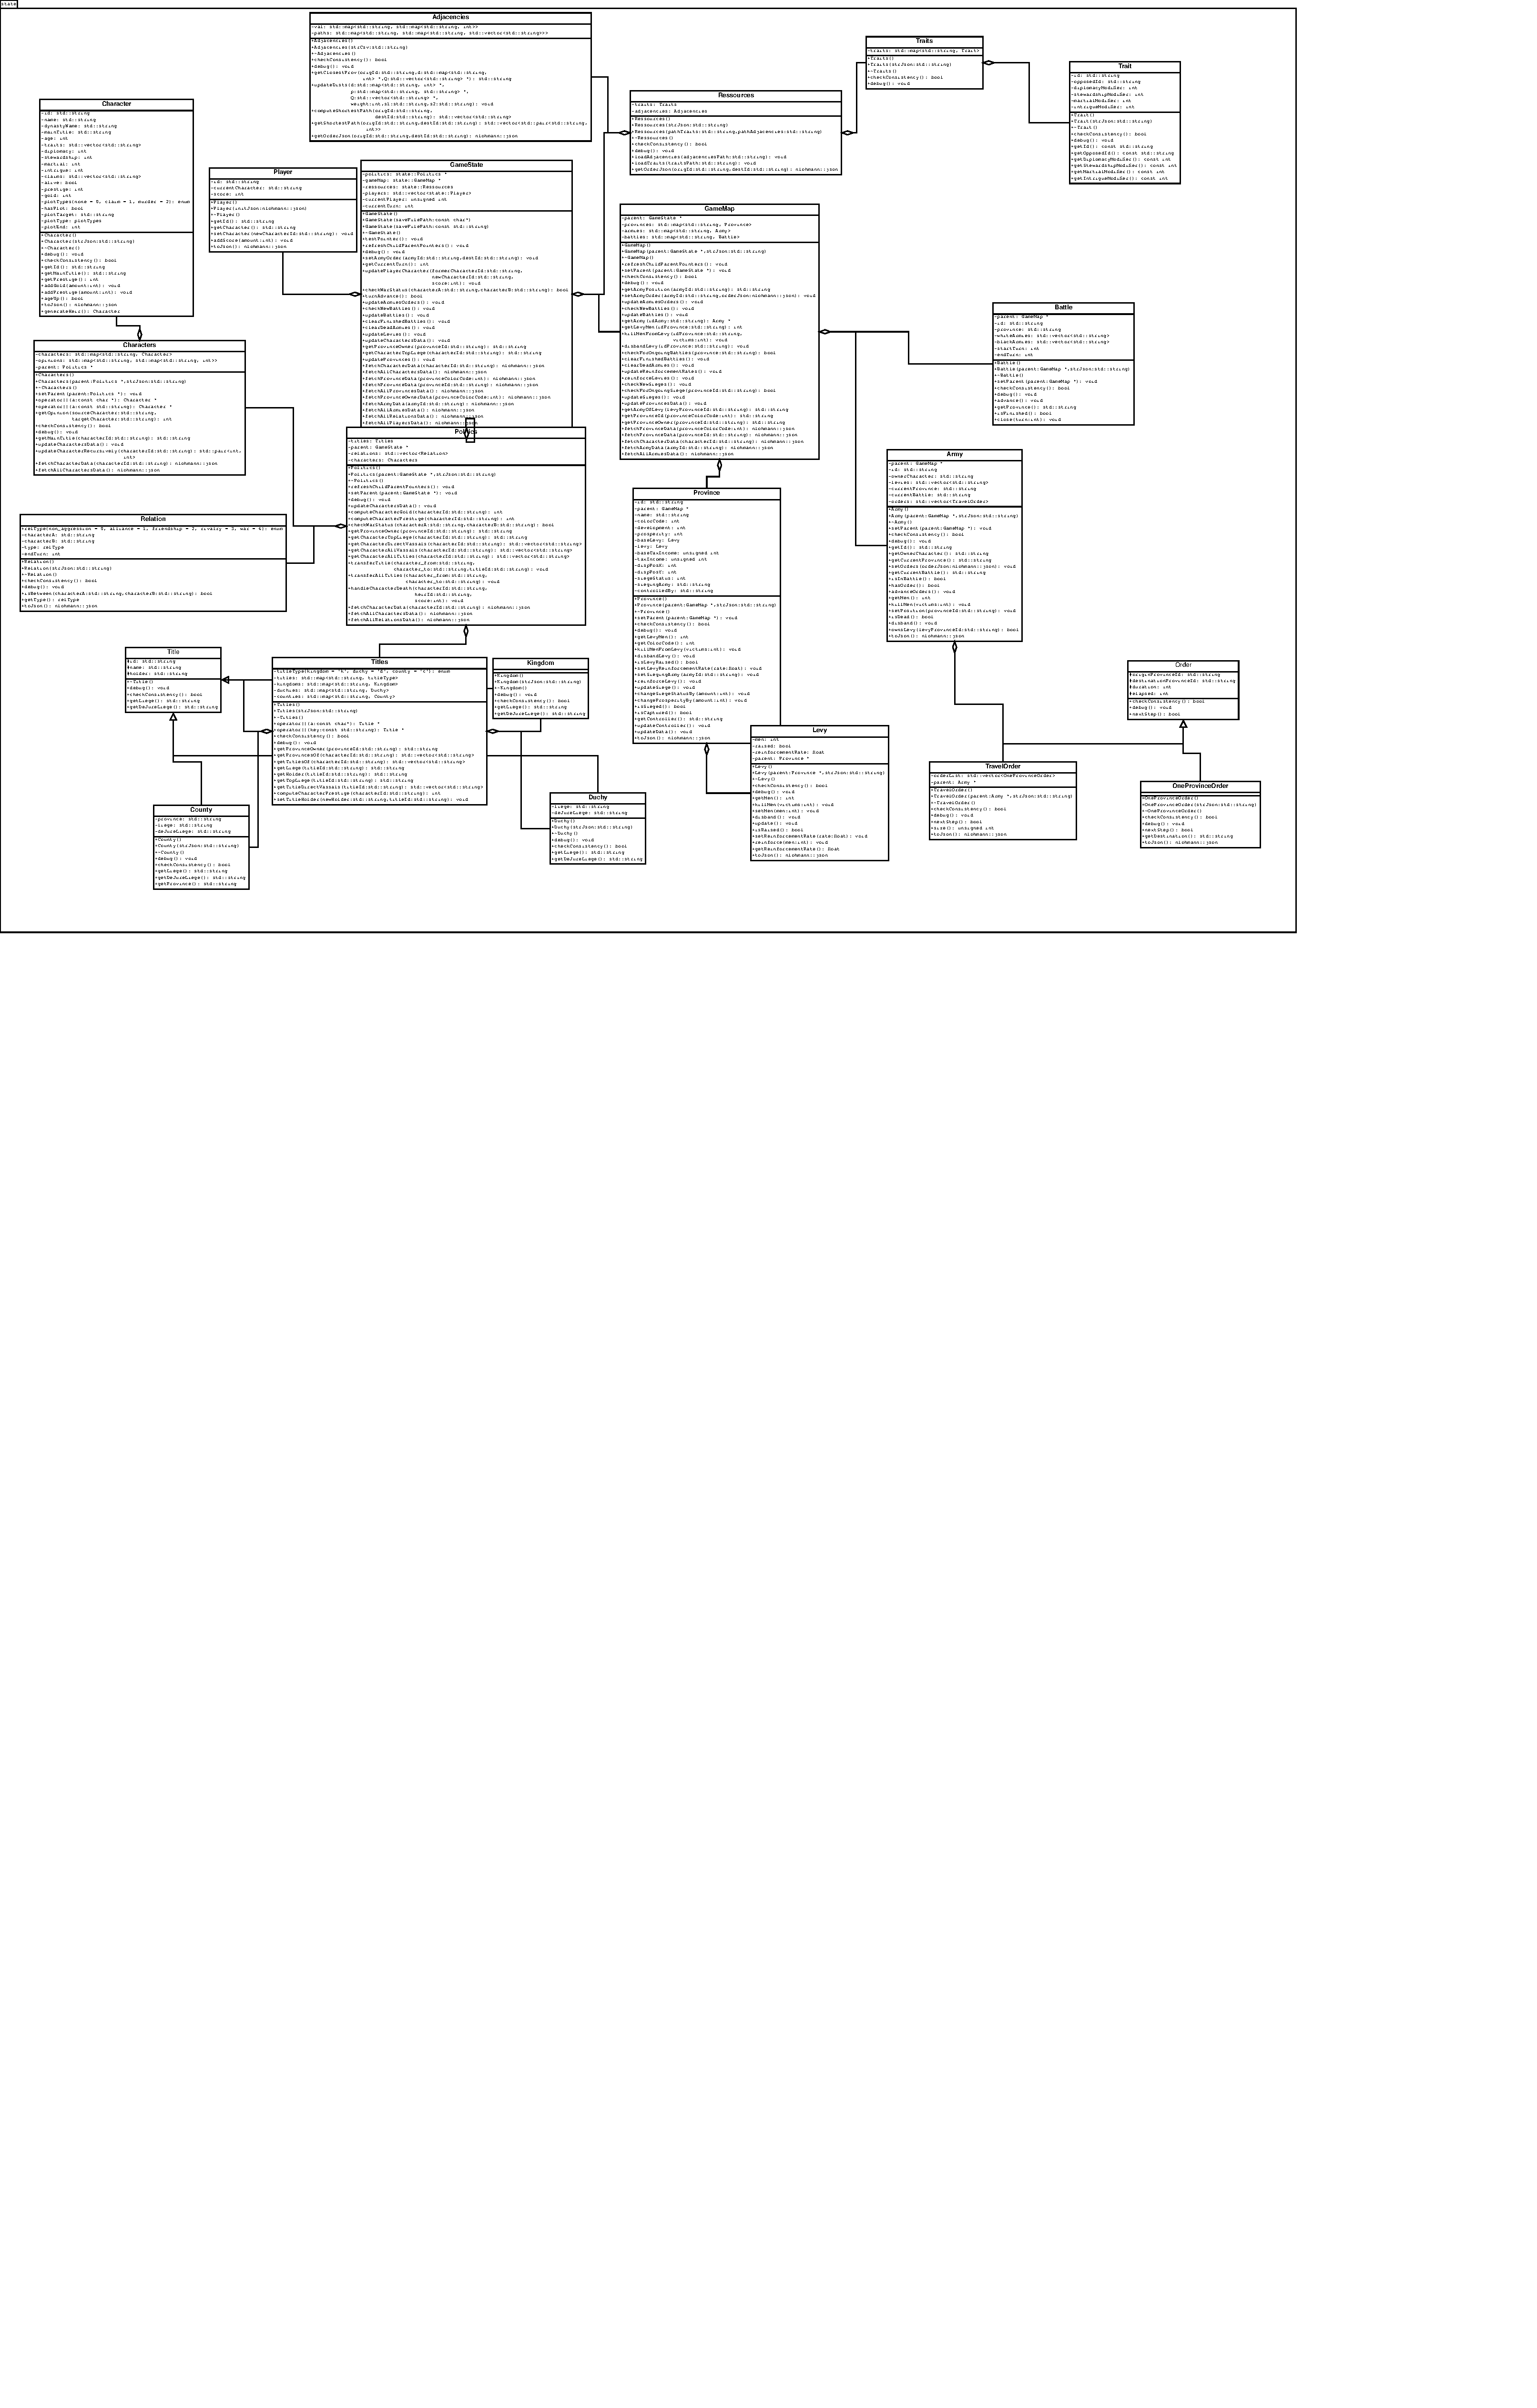
\includegraphics[width=0.9\paperheight]{state.pdf}
\caption{\label{uml:state}Diagramme des classes d'état.} 
\end{figure}
\end{landscape}

\clearpage
\section{Rendu: Stratégie et Conception}

Notre stratégie générale consiste à créer une fenêtre (Window) qui va se rafraîchir régulièrement en utilisant la bibliothèque sfml.\\
Lors du rafraîchissement de la fenêtre, les divers élément composant la page sont affichés.\\

Les élément sont affichés dans des cadres (Frames), eux-mêmes compris dans des Canvas. Les canvas sont placés dans la fenêtre. L'idée est que les Frames peuvent se superposer et potentiellement être ouverts ou fermés à n'importe quel moment, tandis que les canvas sont plus statiques. Cela permet surtout de compartimenter l'affichage.\\

Ces éléments sont ou bien statiques, ou bien liés à des attributs d'objets composant l'état. Dans le second cas, ils décrivent comment afficher ces données.\\
D'autre part certains éléments sont interactifs, c'est-à-dire qu'ils peuvent provoquer des changements graphiques ou bien modifier l'état de jeu lorsqu'on interagit avec eux.
Ainsi cliquer sur une des provinces de la carte ouvre un Frame contenant des cadres de texte (Text) qui décrit l'état de la province en utilisant les informations disponible dans la classe Province des états. Les Frames ainsi créés doivent pouvoir être fermés à tout moment par le joueur à l'aide d'un bouton qui lance le destructeur de l'objet.\\ 
Si un élément doit modifier l'état de jeu, une commande est envoyée au moteur de jeu qui se charge des modifications.\\
L'affichage de la carte du monde se fait à partir de l'objet View de sfml qui permet de n'afficher qu'une partie d'une scène. \\
Les autres éléments sont des rectangles qui contiennent des types de données variables.\\

\subsection{Stratégie de rendu d'un état}

\begin{itemize}
\item Window\\
Description :\\
Le c{\oe}ur de la partie rendu. Cette classe utilise un objet RenderWindow de sfml pour créer une fenêtre. Window comprend aussi une fonction renderLoop() qui va rafraîchir l'affichage régulièrement.\\
Attributs :
\begin{itemize}
\item window de type sf::RenderWindow, la fenêtre affichée
\item width de type int la largeur de la fenêtre
\item height de type int la hauteur de la fenêtre\\
\end{itemize}
\item Canvas\\
Description :\\
Un cadre lié à une fenêtre.\\
Attributs :
\begin{itemize}
\item window de type Window  *, pointeur vers la fenêtre à laquelle appartient le canvas
\item width de type int la largeur du canvas
\item height de type int la hauteur du canvas
\item x de type int la position horizontale du canvas dans la fenêtre
\item y de type int la position verticale du canvas dans la fenêtre\\
\end{itemize}
\item Frame\\
Description :\\
Un cadre lié à un canvas. Des éléments peuvent y être placés.\\
Attributs :
\begin{itemize}
\item canvas de type Canvas *, pointeur vers le canvas auquel appartient le Frame
\item width de type int la largeur du Frame
\item height de type int la hauteur du Frame
\item x de type int la position horizontale du Frame dans le Canvas
\item y de type int la position verticale du Frame dans le Canvas\\
\end{itemize}
\item Element\\
Description :\\
Un élément généraliste dont tous les autres éléments héritent.\\
Attributs :
\begin{itemize}
\item frame de type Frame *, pointeur vers le Frame dans lequel est placé l'élément
\item width de type int la largeur de l'élément
\item height de type int la hauteur de l'élément
\item x de type int la position horizontale de l'élément dans le Frame
\item y de type int la position verticale de l'élément dans le  Frame\\
\end{itemize}
\item interactiveElement\\
Description :\\
Un élément iteractif : décrit les éléments qui déclenchent des réactions lors de certaines actions du joueur. Hérite de la classe Element.\\
Attributs :
\begin{itemize}
\item  N/A \\
\end{itemize}
\item IObserver\\
Description :\\
Une interface d'observer.\\
Attributs :
\begin{itemize}
\item N/A \\
\end{itemize}
\item Button\\
Description :\\
Un bouton. cliquer dessus déclenche une fonction, si le joueur a la possibilité d'effectuer cette action. Hérite de InteractiveElement.\\
Attributs :
\begin{itemize}
\item available de type bool, décrit si le joueur a la possibilité d'effectuer l'action liée au bouton.
\item text de type string, le texte affiché sur le bouton\\
\end{itemize}
\item ObserverButton\\
Description :\\
Observer lié à un bouton, en cas de clic sur le bouton déclenche la fonction associée. Hérite de IObserver.\\
Attributs :
\begin{itemize}
\item N/A\\
\end{itemize}
\item ViewMap\\
Description :\\
Permet de visualiser une partie plus ou moins grande de la carte du monde. Hérite de InteractiveElement.\\
Attributs :
\begin{itemize}
\item zoom de type int, décrit le niveau de zoom par rapport à la carte complète
\item mapX de type int, décrit la position horizontale de ViewMap sur la carte
\item mapY de type int, décrit la position verticale de ViewMap sur la carte\\
\end{itemize}
\item ObserverMap\\
Description :\\
Observer lié à ViewMap, permet d'observer les commandes liées au zoom et au déplacement de la vue dans la carte. Hérite de IObserver.\\
Attributs :
\begin{itemize}
\item N/A\\
\end{itemize}
\item ShowArmy\\
Description :\\
Permet de visualiser une armée sur la carte et d'interagir avec elle. Hérite de InteractiveElement.\\
Attributs :
\begin{itemize}
\item army de type Army, l'armée à laquelle est liée l'objet ShowArmy.\\
\end{itemize}
\item ObserverArmy\\
Description :\\
Observer lié à ShowArmy, permet d'observer les commandes liées à un objet ShowArmy. Hérite de IObserver.\\
Attributs :
\begin{itemize}
\item N/A\\
\end{itemize}
\item Text\\
Description :\\
Cadre contenant du texte. Hérite de Element.\\
Attributs :
\begin{itemize}
\item characterSize de type int, définit la taille du texte affiché dans l'objet Text.
\item displayedText de type std::string, décrit le texte affiché
\item textAdress de type *std::string, l'adresse du texte à afficher\\
\end{itemize}
\item Image\\
Description :\\
Element permettant d'afficher une image fixe. Hérite d'Element.\\
Attributs :
\begin{itemize}
\item keepRatio de type bool, décrit si l'image doit être adaptée aux dimensions de l'objet ou si elle doit garder son ratio
\item followWidth de type bool, dans le cas où keepRatio est vrai, cet attribut permet de décider si l'image doit être adaptée selon la largeur ou la hauteur de l'objet
\item sprite de type sf::sprite, support utilisé pour afficher l'image
\item texture de type sf::texture, variable dans laquelle on charge l'image à afficher\\
\end{itemize}
\end{itemize}

 

\subsection{Conception logiciel}

\begin{landscape}
\begin{figure}[p]
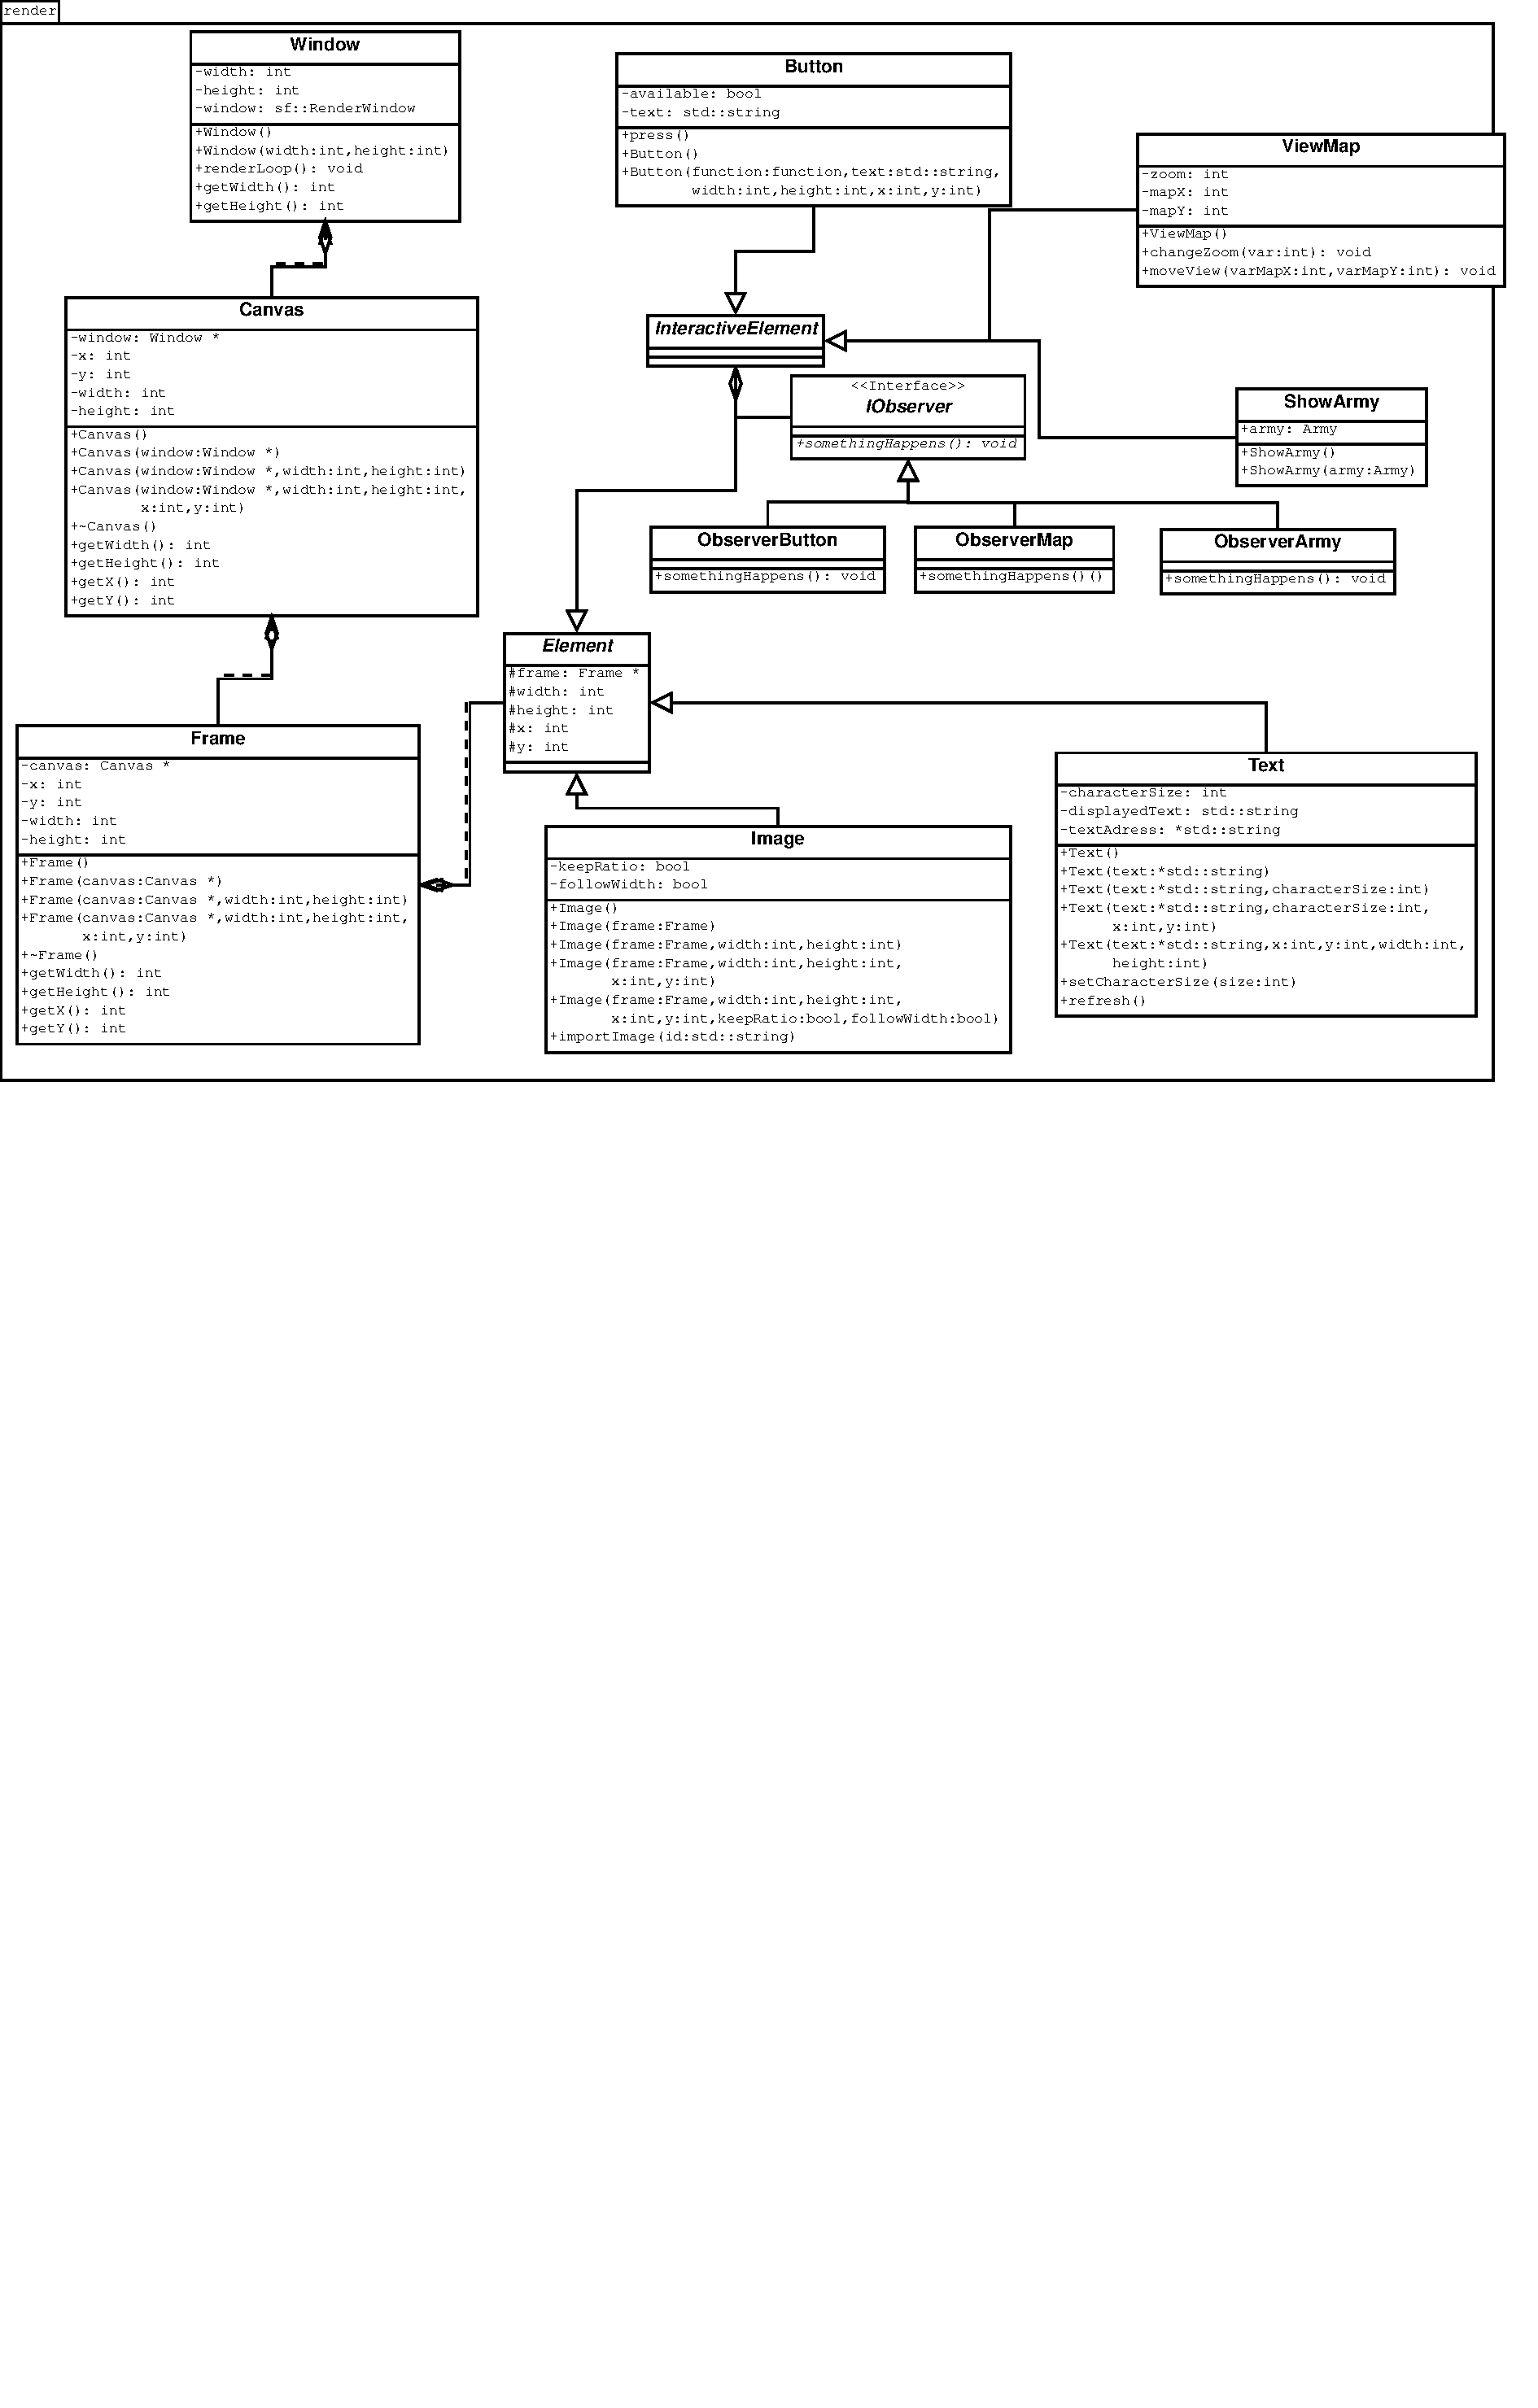
\includegraphics[width=0.9\paperheight]{render.pdf}
\caption{\label{uml:render}Diagramme des classes de rendu.} 
\end{figure}
\end{landscape}

\clearpage
\section{Règles de changement d'états et moteur de jeu}

\subsection{Règles}

\clearpage
\subsection{Conception logiciel}


%\begin{landscape}
%\begin{figure}[p]
%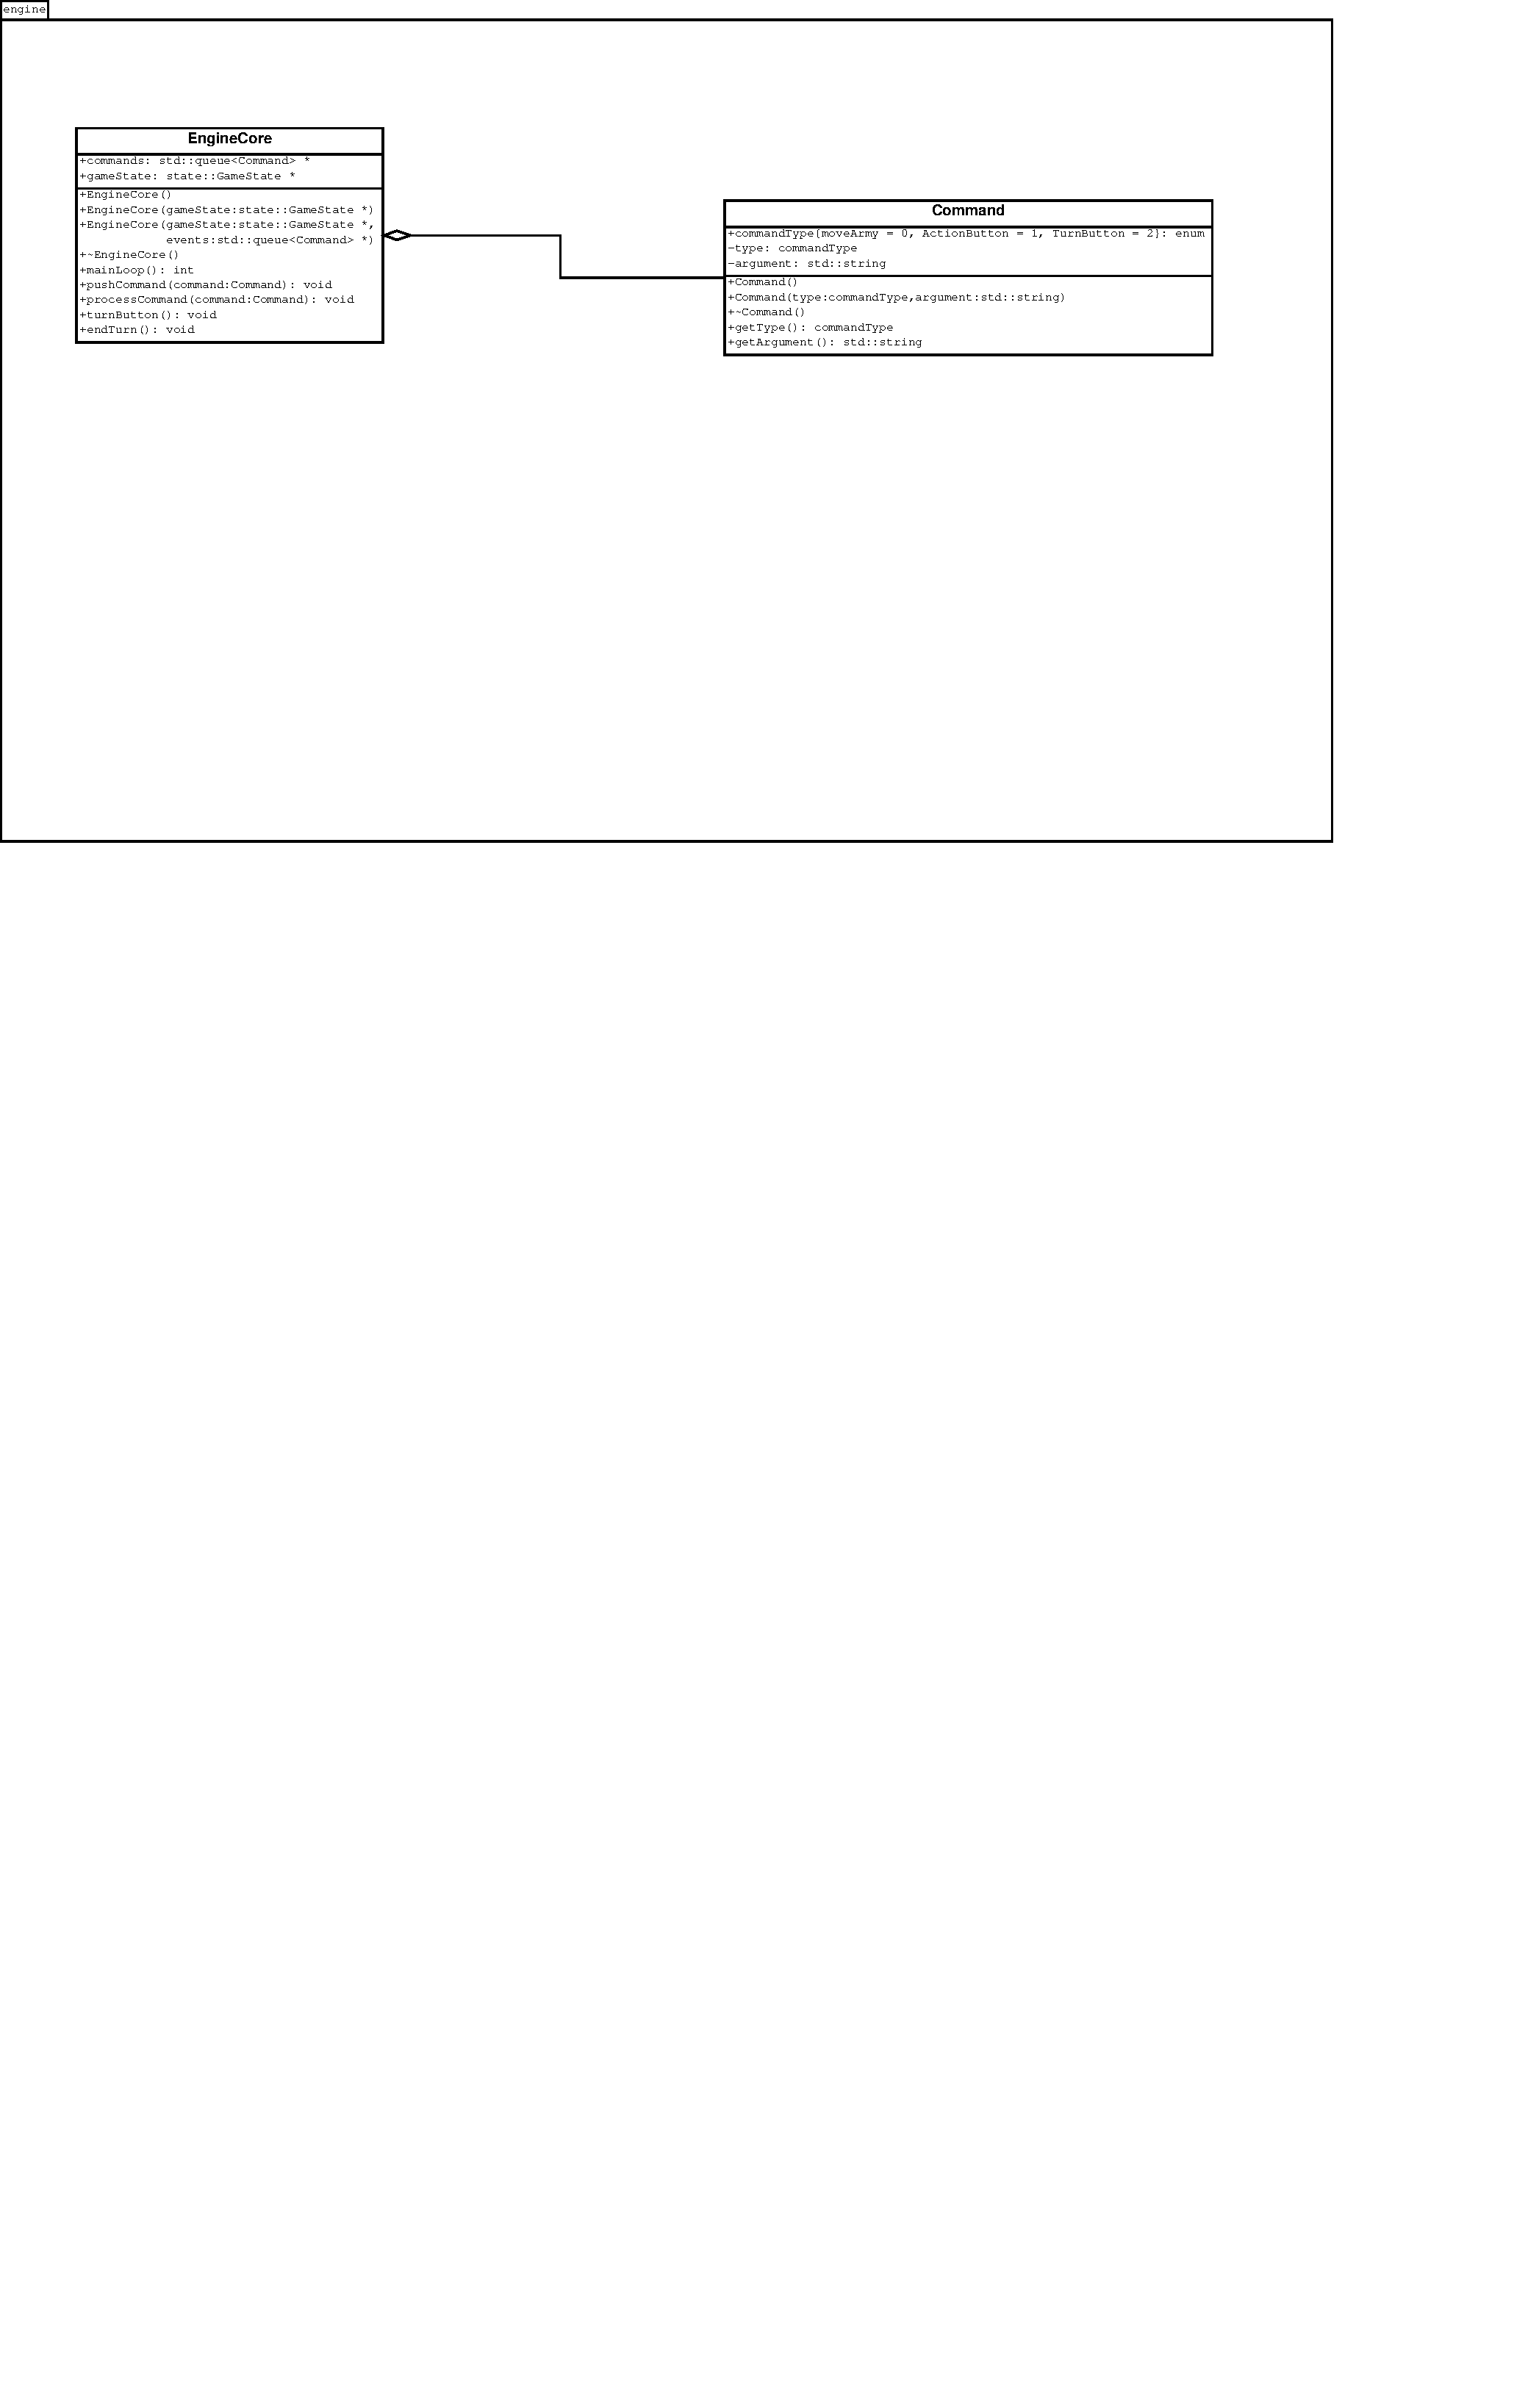
\includegraphics[width=0.9\paperheight]{engine.pdf}
%\caption{\label{uml:engine}Diagramme des classes de moteur de jeu.} 
%\end{figure}
%\end{landscape}


\section{Intelligence Artificielle}

\subsection{Stratégies}

\clearpage
\subsection{Conception logiciel}


%\begin{landscape}
%\begin{figure}[p]
%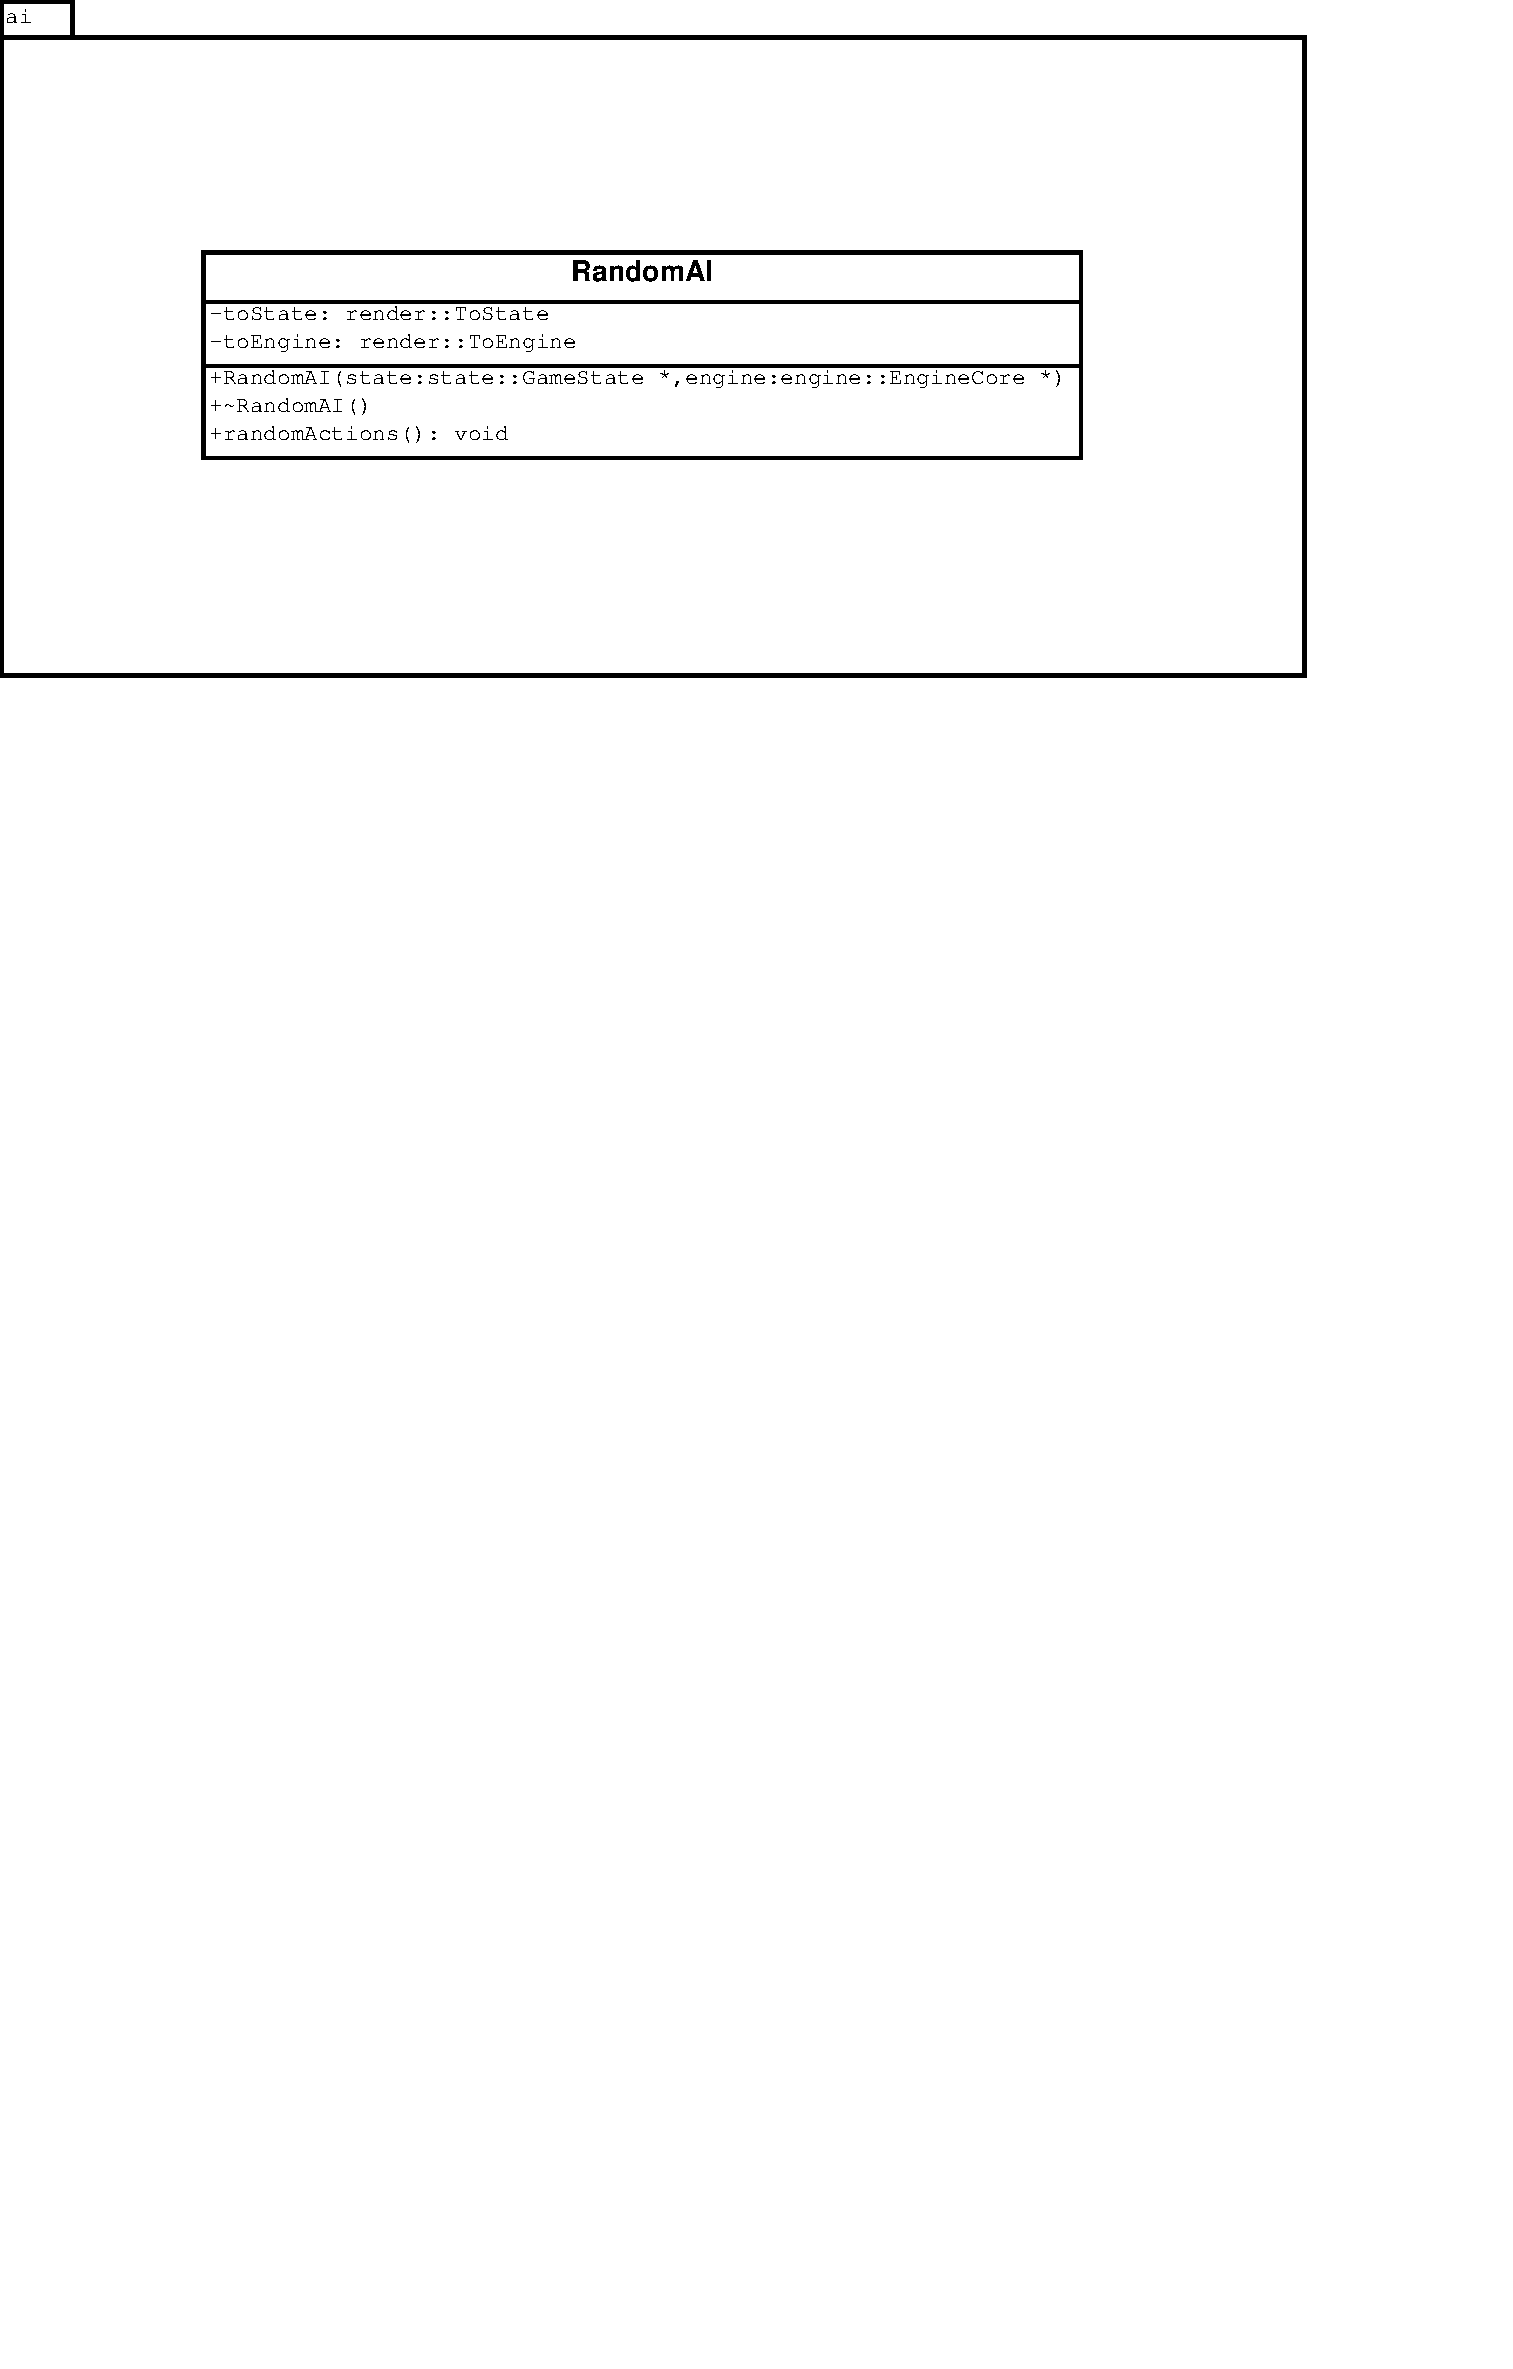
\includegraphics[width=0.9\paperheight]{ai.pdf}
%\caption{\label{uml:ai}Diagramme des classes d'intelligence artificielle.} 
%\end{figure}
%\end{landscape}


\section{Modularisation}
\label{sec:module}

\subsection{Organisation des modules}

\clearpage
\subsection{Conception logiciel}


%
%\begin{landscape}
%\begin{figure}[p]
%\includegraphics[width=0.9\paperheight]{module.pdf}
%\caption{\label{uml:module}Diagramme des classes pour la modularisation.} 
%\end{figure}
%\end{landscape}

\end{document}
